\documentclass[12pt,oneside,a4paper]{article}
\usepackage[margin=2.5cm]{geometry}
\usepackage{fancyhdr}
\usepackage{amsmath,amsthm,amssymb}
\usepackage{graphicx}
\usepackage[hidelinks]{hyperref}
\usepackage[dvipsnames]{xcolor}

\usepackage{mathtext}
\usepackage[style=numeric, backend=biber]{biblatex}
\addbibresource{reference.bib}

\usepackage[T1,T2A]{fontenc}
\usepackage[utf8]{inputenc}
\usepackage[english,bulgarian]{babel}
\usepackage{setspace}
\usepackage{extarrows}
\usepackage{titling}
\usepackage{enumitem}
\date{}
\newtheorem{problem}{Задача}
\newtheorem{subproblem}{Задача}[problem]
\newtheorem*{solution}{Решение}

\setlength{\parindent}{10pt}
\setlength{\parskip}{1ex}

\setlength{\droptitle}{4\baselineskip}
\setlength{\bibitemsep}{1.5\baselineskip}

\addto\captionsbulgarian{%
	\renewcommand{\figurename}{Фигура} % Rename figure captions
	\renewcommand{\tablename}{Таблица} % Rename table captions
}

\title{\includegraphics[width=0.15\linewidth]{SU.png} \hspace{0.3\linewidth} \includegraphics[width=0.15\linewidth]{FMI.png}\vspace{2cm} \\\Huge Доклад\\\Large към курсов проект на тема\\\Huge \vspace{1cm}\textbf{ Невронен машинен превод чрез генеративен езиков модел}\\\vspace{.5cm}\Large\textit{Търсене и извличане на информация}\\зимен семестър, 2024/2025 г.}
\author{Калоян Цветков\\4MI0800017}
\date{14.02.2025г.}

\begin{document}
	
	\begin{titlingpage}
		\maketitle
	\end{titlingpage}
	

	\section{Резюме}\mbox{}
	
	Проектът цели реализация на модел за едновремено генериране на последователност на английски по зададен префикс, както и преводът ѝ от английски на български. Моделът е обучаван единствено върху предоставените тренировъчни данни. Предадените скриптове включват настройка на модела, довършване по дадена начална последователност и превод на цял корпус на български.
	
	Сред предадените файлове присъства и т.н. \textit{jupyter notebook} на име \textbf{TII\_project.ipynb}, където има посочени конкретни команди за работа с проекта.
	
	\section{Архитектура}\mbox{}
		
	За предварителната обработка на текстовите данни се използва вграден токенизатор от библиотеката \texttt{tokenizers}. Вграденият токенизатор осигурява бърза и оптимизирана обработка на текста, като прилага предварително обучени алгоритми за сегментиране на думите. Началните опити с посимволно влагане и влагане по думи имаха проблеми съответно трудно научаване на зависимости между цели думи и прекалено голям речник. Експериментите със собствената имплементация на генериране на токени, кодиране и декодиране на текст показаха, че липсата на умения за паралелизация на токенизирането на множество данни увеличава значително времето за изпълнение и я правят неизползваема. Предоставен е скрипт \texttt{generateTokens.py}, генериращ конкретен брой токени, както и примерен изход (\texttt{tokens.json}) върху тренировъчното множество.
		
	Моделът представлява невронна мрежа за езиково моделиране, базирана на трансформър архитектурата, предложена в \textbf{\cite{vaswani2017attention}}. Той използва трансформър енкодери, които включват механизъм за самообучение (\textit{self-attention}), което позволява паралелната обработка на входни последователности.
	
	Основната структура на модела включва слой \texttt{torch.nn.Embedding}, който преобразува думите в числови вграждания. След това тези вграждания се обогатяват с позиционен енкодинг, който се използва, за да се добави информация за реда на думите в последователността. Използваният позиционен енкодинг е имплементираният на упражнения чрез клас \texttt{PositionalEncoding}.
	
	В същината на модела се намира енкодер, използващ архитектура \textit{трансформър}, реализиран чрез \texttt{TransformerEncoder} от \texttt{PyTorch}, представляващ многослойно наслагване на \texttt{TransformerEncoderLayer}, реализиращ описаната в  \textbf{\cite{vaswani2017attention}} архитектура. Важно е използването на маска, представена чрез горно триъгълна матрица, скриваща информация за следващи последователности. Според описаното в \textbf{\cite{vaswani2017attention}}, най-добро представяне се постига, когато размерността на скрития слой на \textit{feed-forward} мрежата е $4$ пъти по-голяма от размера на влагането, поради което така е постъпено и тук. Чрез линейна проекция, изхода от трансформъра се преобразува в разпледеление на думите от речника. Използвана е емпирична крос ентропия като функция за загуба при обучението.
	
	Моделът също така включва механизъм за генерация на текст, като използва семплиране с температурен коефициент за регулиране на разпределението на вероятностите при генериране на следваща дума. При стартиране на генерацията моделът използва даден префикс и генерира нови думи (чрез семплиране) последователно, докато не достигне зададения лимит или не генерира специален (\textit{end}) токен.
	
	
	\section{Източници}
	
	\begin{itemize}
		\item Официална документация към \texttt{TransformerEncoderLayer} от \texttt{PyTorch}:\\ \href{https://pytorch.org/docs/stable/generated/torch.nn.TransformerEncoderLayer.html}{https://pytorch.org/docs/stable/generated/torch.nn.TransformerEncoderLayer.html}
		\item Официална документация към \texttt{TransformerEncoder} от \texttt{PyTorch}:\\ \href{https://pytorch.org/docs/stable/generated/torch.nn.TransformerEncoder.html}{https://pytorch.org/docs/stable/generated/torch.nn.TransformerEncoder.html}
	\end{itemize}
	
	\printbibliography
	
	
	\section{Процес на обучение}
	
	Подготовката на корпус, а след това и обучение се извършват стандартно чрез аргументите съответно \texttt{prepare} и \texttt{train}/\texttt{extratrain} на програмата \texttt{run.py} при наличие на \textit{json} файл с токени\\ (\texttt{tokensFileName}).\\ Ако такъв няма е необходимо предварително изпълнение на прорамата (\texttt{generateTokens.py}).
	
	Обучението на предадения модел е извършено на графична карта \textit{T4}, предоставена от платформата \textit{Google Colab}. Тази платформа предлага безплатен достъп до \textit{GPU} ресурси, което позволява по-бързо и ефективно обучение на дълбоки невронни мрежи.

	
	Следните хиперпараметри бяха използвани за обучението на модела:
	
	\begin{itemize}
		\item \textbf{Параметри на модела:}
		\begin{itemize}
			\item Размер на влагането (\texttt{d\_model}) е зададен на 128
			\item Размерът на скрития слой на \textit{feed-forward} частта е зададен на 512
			\item 8 глави на вниманието (\texttt{n\_heads})
			\item 4 слоя на вниманието (\texttt{num\_layers})
		\end{itemize}
		\item \textbf{Скорост на обучение:} Скоростта на обучение е зададена на 0.001 (\texttt{learning\_rate}).
		\item \textbf{Размер на партидата:} 32 (\texttt{batchSize}).
		\item \textbf{Нормата на градиентите} се ограничава до максимална стойност от 10.0 (\texttt{clip\_grad}).
		\item \textbf{Логване:} На всеки 10 стъпки от обучението (\texttt{log\_every}) в конзолата се извежда текущото състояние на обучението, като то се записва на всеки 200 стъпки (\texttt{log\_file\_every}) в посочен файл (\texttt{log\_filename}). Тестовете за перплексия се изпълняват също на всеки 200 стъпки (\texttt{test\_every}).
	\end{itemize}
	
	
	\section{Резултати}
	
	След приблизително $7$ часа обучение моделът достига перплексия $\textbf{4.704}$ и \textit{BLEU} резултат от $\textbf{41.865}$ върху тестовото множество данни. Резултатите по време на обучението според итерациите с посочения размер на партида са изложени в Таблица \ref{table:training_results} на всеки $50000$ итерации, както и на всяки $200$ във Фигура \ref{fig:loss} и Фигура \ref{fig:perplexity}.
	
	\begin{table}[h]
		\centering
		\begin{tabular}{|c|c|c|c|}
			\hline
			\textbf{Итерация}  & \textbf{Загуба} & \textbf{Думи/сек} & \textbf{Най-добра перплексия} \\
			\hline
			50 000 & 1.988 &36890.72 & 6.235\\
			100 000 &1.977 &38979.05 &5.548\\
			150 000 &1.645 &37719.01 &5.296\\
			200 000 &1.773 &34864.27 &5.153\\
			250 000 &1.918 &38086.78 &5.074\\
			300 000 &1.704 &35146.69 &5.016\\
			350 000 &1.685 &34397.45 &4.967\\
			400 000 &1.780 &31387.54 &4.923\\
			450 000 &1.692 &39530.54 &4.907\\
			500 000 &1.725 &39798.69 &4.895\\
			550 000 &1.542 &33088.33 &4.871\\
			600 000 &1.676 &37576.14 &4.864\\
			650 000 &1.907 &40292.59 &4.847\\
			650 000 &1.731 &30246.79 &4.847\\
			700 000 &1.623 &34977.17 &4.743\\
			749 200 &1.563 &36504.24 & 4.704\\
			\hline
		\end{tabular}
		\caption{Резултати от обучението}
		\label{table:training_results}
	\end{table}\newpage
	\begin{figure}[ht]
		\centering
		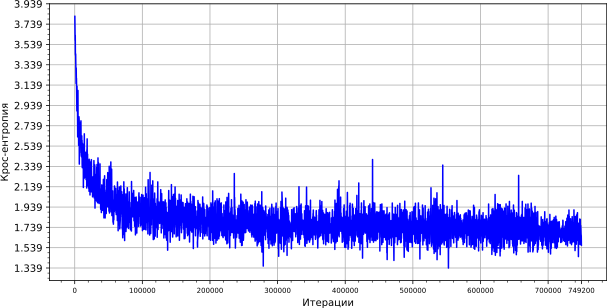
\includegraphics[width=0.9\linewidth]{loss.pdf}
		\caption{Отношение на крос-ентропия спрямо броя итерации}
		\label{fig:loss}
	\end{figure}
	\begin{figure}[ht]
		\centering
		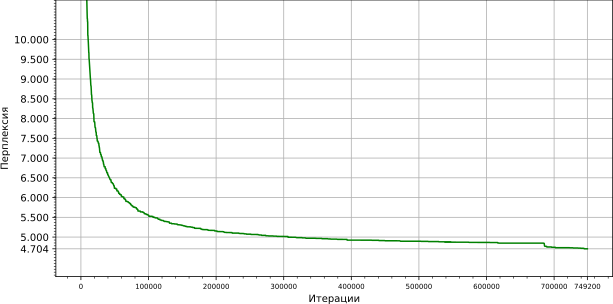
\includegraphics[width=0.9\linewidth]{perplexity.pdf}
		\caption{Отношение на перплексията спрямо броя итерации}
		\label{fig:perplexity}
	\end{figure}
	
	\section{Заключение}
	
	Моделът \textbf{NMTmodel}, постигащ BLEU резултат от приблизително $41.8$, се спрява задоволително както със задачата за довършване на последователност на английски, така и със задачата за превод на последователност на английски на български, при това едновремено. Тематиката на трнировъчните данни ограничават модела в някаква степен до добър превод предимно на публицистични текстове.
	
	Бъдещи подобрения включват паралелизация на токенизирането на корпус с цел употреба на токени, създадени от скрипт на автора, както и паралелизиран превод на корпус.
	
	
	
\end{document}
